\chapter{REQUIREMENT ANALYSIS AND DESIGN}
\section{Introduction}This chapter walks through the requirement analysis and design phases of the LexiFlow project. It's basically the groundwork for building a well-organised language learning system meant for the UTM community. The approach here is methodical: we pin down and study what different stakeholders really need, and we do that through structured stuff like surveys and interviews; once the requirement analysis is done, the chapter moves on to designing the system. Part of that means working out a system architecture that lets LexiFlow's different parts talk to each other smoothly. So we map out the modular structure, figure out how those modules communicate, and produce sure the whole architecture lines up with what the project set out to achieve for starters.
\section{Requirements Gathering and Analysis}We dug into the LexiFlow requirements pretty carefully, mostly through an interview with the stakeholders over at UTM Language Academy. That part mattered. It helped us spell out where the existing system falls short and what these stakeholders actually want from the proposed LexiFlow platform. What they told us made one thing clear: they badly need an automated tool that can handle real Mandarin content and hand learners synchronized audio, pinyin, and English translations all at once. During the analysis, we leaned harder on a handful of features that seemed key to making the system genuinely useful. Stuff for user evaluation, like flashcards and quizzes, plus themed playlists that retain the learning more organized and structured. We're expecting these to smooth out the whole learning process. Figure~\ref{fig:use_case} below lays out the use case diagram of LexiFlow with everything mentioned above. \begin{figure}[h!]
    \centering
    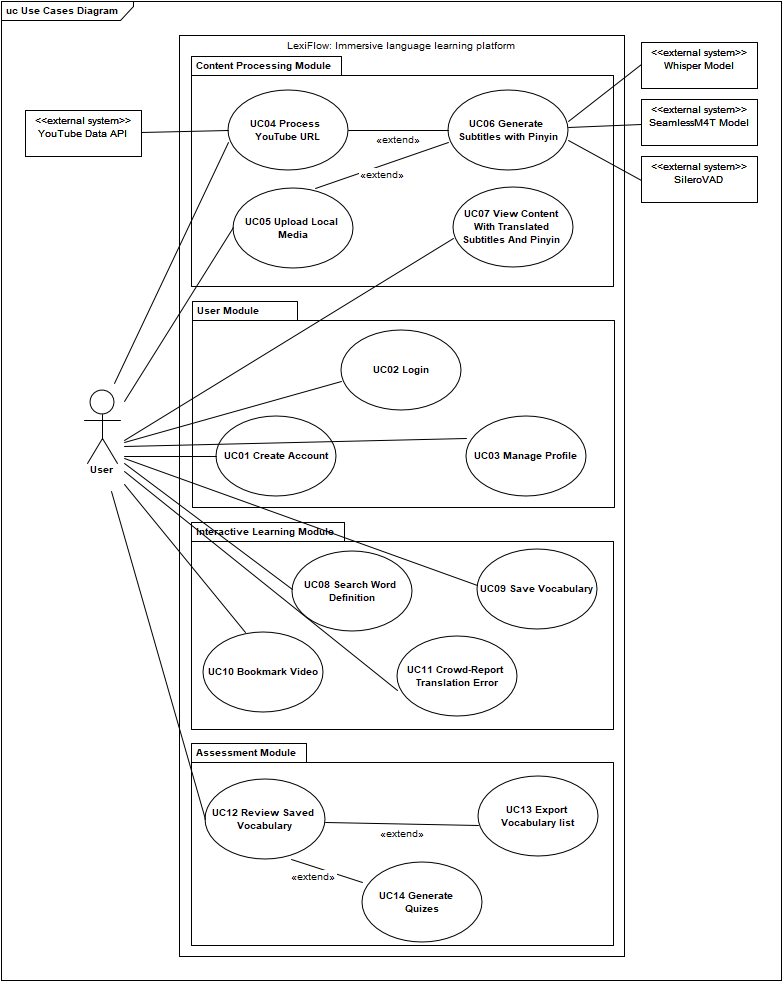
\includegraphics[width=0.8\textwidth]{./figs/use_cases.png}
    \caption{Use Case Diagram of LexiFlow}\label{fig:use_case}
\end{figure} So the requirement analysis wrapped up with a solid grip on the system specs and what it needs to do. These requirements are meant to steer the later phases, the design and the actual building of the system. The project's being built on purpose to match what the UTM community needs and expects, but LexiFlow also aims to fix the gaps in the current setup while adding new features that improve user experience and safety. And that kind of approach should give us a final product that's genuinely tailored to what the UTM community is asking for.
\subsection{Functional Requirements}The functional requirements of LexiFlow come from the use case diagram (Figure~\ref{fig:use_case}) and are laid out in Table~\ref{tab:functional_requirements}. \begin{longtable}{>{\centering\arraybackslash}m{1.2cm} >{\centering\arraybackslash}m{3cm} >{\arraybackslash}m{8cm}} \caption{Functional Requirements of LexiFlow System}\label{tab:functional_requirements} \\ \toprule \textbf{ID} & \textbf{Name} & \textbf{Description} \\ \midrule \endfirsthead \multicolumn{3}{l}{\textit{(Continued from previous page)}} \\ \toprule \textbf{ID} & \textbf{Name} & \textbf{Description} \\ \midrule \endhead \midrule \multicolumn{3}{r}{\textit{(Continued on next page)}} \\ \endfoot \bottomrule \endlastfoot UC01 & Create Account & Allows new users to register and create an account in the system. \\ UC02 & Login & Enables registered users to authenticate and access the system. \\ UC03 & Manage Profile & Allows users to view and update their personal information and preferences. But \\ UC04 & Process YouTube URL & Handles the processing of YouTube video URLs for content extraction. \\ UC05 & Upload Local Media & Enables users to upload media files from their local device for processing. \\ UC06 & Generate Subtitles & Automatically creates subtitles for processed video content. \\ UC07 & Find Translated Content & Provides functionality to locate translated versions of content. \\ UC08 & Search Word Definition & Allows users to search for definitions of words within the learning module. \\ UC09 & Save Vocabulary & Enables users to save new vocabulary words for later review. \\ UC10 & Bookmark Video & Allows users to bookmark specific video segments for future reference. \\ UC11 & Crowd-Report Translation Error & Provides a mechanism for users to collaboratively report translation errors. \\ UC12 & Review Saved Vocabulary & Enables users to review and practice vocabulary they have previously saved. \\ UC13 & Export Vocabulary list & Allows users to export their vocabulary lists for use outside the system. \\ UC14 & Generate Quizes & Automatically creates quizes from saved vocabulary for study purposes. Take the use case for processing YouTube URLs (UC04) as an example, shown in Table~\ref{tab:use_case_uc04}. It brings in a couple of key actors, namely the user and the YouTube Data API. To pull the video content, the system validates the URL, grabs the metadata, and checks how long the video runs. Every use case is fully written up in the Software Requirements Specification (SRS). That includes the normal flow, the alternative flows (think invalid duration or restricted content), and the exception flows too. You'll find the complete use case specs in Appendix~\ref{app:srs}.
\begin{longtable}{|>{\columncolor[HTML]{D9D9D9}}l|p{10cm}|} \caption{Use Case Description for UC04 \textless{}Process YouTube URL\textgreater{}}\label{tab:use_case_uc04} {} \\ \hline \textbf{Use Case ID} & UC04 \\ \hline \textbf{Use Case Name} & Process YouTube URL \\ \hline \textbf{Description} & Lets a logged-in user drop in a YouTube video URL so LexiFlow can handle the transcription, translation, and lined-up subtitle generation on its own. \\ \hline \textbf{Actor(s)} & User, YouTube Data API \\ \hline \textbf{Pre-conditions} & 1. The user is logged into their LexiFlow account. \\ & 2. LexiFlow can get online to reach YouTube. \\ & 3. There's an active connection to the YouTube Data API. \\ \hline \textbf{Normal Flow (NF)} & 1. User heads to the "Upload/Process Content" section \\ & 2. User picks the option to process a YouTube URL \\ & 3. User types in a valid YouTube video URL \\ & 4. User submits the URL for processing \\ & 5. System checks the URL and pulls the video stream \\ & 6. System kicks off the content processing pipeline \\ & 7. System lets the user know processing has started \\ \hline \textbf{Alternative Flow (AF)} & AF1: Invalid YouTube URL \\ & \quad 1. If the URL's invalid or the video can't be found: \\ & \quad \quad 1.1 System shows an "Invalid YouTube URL" error \\ & \quad \quad 1.2 Asks the user to enter the correct URL \\ & AF2: Restricted/Private Video \\ & \quad 1. If the video is region-locked or private: \\ & \quad \quad 1.1 System shows an access restriction error \\ & \quad \quad 1.2 Use case ends without success \\ \hline \textbf{Exception Flow (EF)} & EF1: Processing Pipeline Failure \\ & \quad 1. If something breaks badly during content processing: \\ & \quad \quad 1.1 System logs the detailed error \\ & \quad \quad 1.2 Shows a generic failure message \\ & \quad \quad 1.3 Use case ends without success \\ & EF2: Network Error During Fetch \\ & \quad 1. If a network hiccup stops the video from being fetched: \\ & \quad \quad 1.1 System shows a network error message \\ & \quad \quad 1.2 Asks the user to check their connection \\ & \quad \quad 1.3 Use case ends without success \\ \hline \textbf{Post-conditions} & 1. The YouTube video content gets pulled successfully \\ & 2. The content processing pipeline is up and running \\ & 3. The user gets a processing status notification \\ \hline \textbf{Special Requirements} & 1. System can get online to reach YouTube \\ & 2.
\subsection{Non-Functional Requirements}Non-functional requirements spell out the quality attributes, system performance, and limits that LexiFlow has to live up to. They're what keeps the system dependable, easy to use, and maintainable over time. You'll find them laid out in Table~\ref{tab:non_functional_requirements}. \begin{longtable}{>{\centering\arraybackslash}m{1.2cm} >{\centering\arraybackslash}m{3cm} >{\arraybackslash}m{8cm}} \caption{Non-Functional Requirements} \label{tab:non_functional_requirements} \\ \hline \textbf{ID} & \textbf{Type} & \textbf{Description} \\ \hline \endfirsthead \multicolumn{3}{l}{\textit{(Continued from previous page)}} \\ \hline \textbf{ID} & \textbf{Type} & \textbf{Description} \\ \hline \endhead \hline \multicolumn{3}{r}{\textit{(Continued on next page)}} \\ \endfoot \hline \endlastfoot NFR-001 & Performance & The system shall process and validate YouTube URLs within 3 seconds to ensure responsive user experience. NFR-002 & Localization & The system shall support display text in at least two languages: English and Mandarin. NFR-003 & Backup & System data shall be backed up automatically every 24 hours and stored securely \\
\end{longtable}
\section{Architectural Design}The Pipe and Filter pattern breaks processing into a chain of separate pieces, the filters, that connect through pipes. Each filter does one specific transformation on the data, then hands the result down the line to the next one. You get better scalability, easier maintenance, and reuse out of this, since filters can be built, tested, and swapped on their own. Keeping concerns separate also makes debugging less painful and leaves room for extending the system later. For LexiFlow's audio processing, this pattern fits really well. Each filter takes care of one job, things like voice activity detection, speech recognition, translation, and pinyin generation. Because of that modularity, you can drop in new steps or replace old ones without touching the rest of the architecture. As shown in Figure~\ref{fig:pipe_and_filter}, the LexiFlow system architecture consists of several key components: \begin{enumerate}[label= (\alph*)] \item \textbf{User Interface (UI):} The front-end application built with Vue.js, providing an interactive platform for users to upload media, view subtitles, and manage vocabulary. Considered as the source of data in the Pipe and Filter architecture. \item \textbf{Backend Services:} roll outed using Node.js and FastAPI, these services handle user requests, process audio and video content, and are considered as pipes in the Pipe and Filter architecture. \item \textbf{Audio Processing Pipeline:} A series of filters that perform tasks such as voice activity detection (SileroVAD), automatic speech recognition (Whisper), translation (painlessM4Tv2), and pinyin generation. \item \textbf{Database:} MongoDB is used to store user profiles, processed content metadata, subtitles, and vocabulary lists. Considered as the sink of data in the Pipe and Filter architecture. \begin{figure}[H]
    \centering
    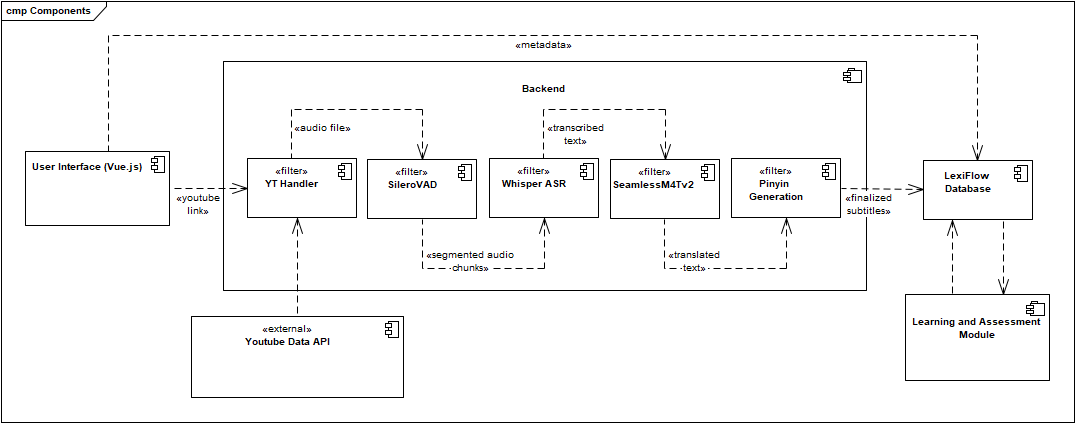
\includegraphics[width=0.95\textwidth]{./figs/arch.png}
    \caption{LexiFlow System Architecture}\label{fig:pipe_and_filter}
    \smallskip
    \begin{flushleft}
        \small * The figure illustrates the Pipe and Filter architecture of LexiFlow, showing the modular processing components and their interactions.
    \end{flushleft}
\end{figure}
\section{Chapter Summary}Chapter 4 of the thesis works through requirement analysis and system design for LexiFlow, laying out how we approached building a language learning platform. It opens by digging into what stakeholders actually need, gathered through interactive sessions. That groundwork feeds the detailed documentation in the Software Requirements Specification (SRS, Appendix~\ref{app:srs}) and Software Design Document (SDD, Appendix~\ref{app:sdd}). From there it covers the pipe-and-filter architecture, which keeps things scalable and efficient, and then the user interface design that makes interaction smoother and ties the whole system together. The point of all this? Lining up with the project's goals while building a solid base for getting LexiFlow up and running. Testing came later. The system was checked through automated end-to-end testing and User Acceptance Testing, covered in Chapter 5 and Appendices~\ref{app:test-execution-report} and~\ref{app:uat-report}, instead of a separate, standalone Software Test Document.
